\documentclass[../main.tex]{subfiles}

% 2.2.1 Wellenverhalten bei Substanzen
Beim zusammenkommen einer Welle mit einer Substanz kann es zu verschiedenen Abschwächungen der Welle kommen. Es spielen Absorption, Streuung, Beugung und Reflexion (Abb. \ref{fig:extinktion_typen}) eine Rolle.

% TODO alternative image (copyright..)
\begin{figure}[ht]
    \centering
    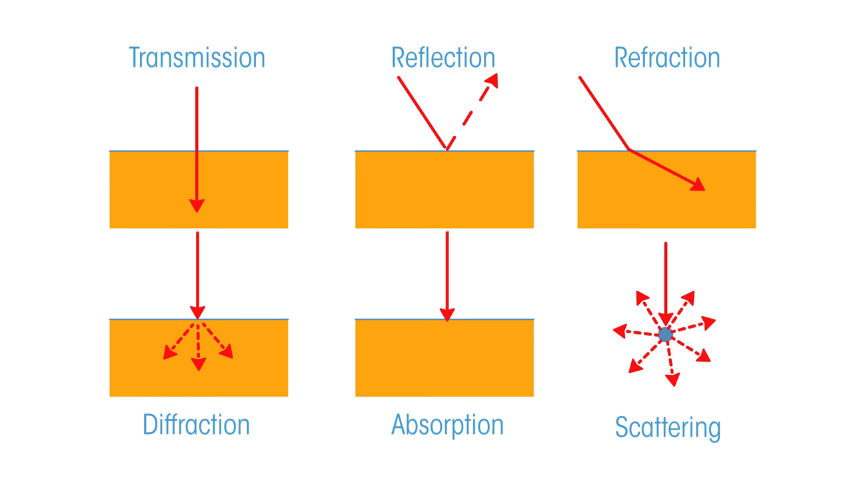
\includegraphics[width=0.65\textwidth]{extinktion_typen.png}
    \caption{Einflussfaktoren auf Extinktion}
    \label{fig:extinktion_typen}
\end{figure}

% 2.2.2 Absorption
\textbf{Absorption} beschreibt in der Physik die Aufnahme von Wellen in einer Substanz.
% 2.2.3 Streuung
\textbf{Streuung} ist die Ablenkung von Wellen in mehrere Richtungen.
% 2.2.4 Beugung
Wenn Strahlungen eine Substanz mit unterschiedlicher Dichte durchqueren, kommt es zu einer Verlangsamung der Ausbreitung, und damit zu einer Richtungsänderung - das ist \textbf{Beugung}.
% 2.2.5 Reflexion
Glatte Oberflächen \textbf{reflektieren} häufig Strahlungen (z.B. Spiegel).